\newthought{The rules determining} thromboelastography results are more complicated than any of the other test within Cerner. In order to ensure the accuracy of the results being verified, the platelet mapping calculations will not be performed until \textit{after} the measured values have been verified.

\bigskip

\newthought{Required training} before proceeding with this section%
\marginnote{This guide assumes that the user is familiar with these functions}.
\begin{itemize}
   \item Cerner App-Bar
   \item Accession Result Entry
   \item Discern Notifications
 \end{itemize}

\section{Procedure}

\paragraph{Open} Accession Result Entry and enter the Accession number of the TEG to be resulted\\
\paragraph{Select} the ``Specimen Type'' from the drop down menu.\\
\vspace{.5em}
\begin{minipage}{\textwidth}
 % trim={<left> <lower> <right> <upper>}
 \IfFileExists{fileA.tex}{\input{fileA.tex}}

  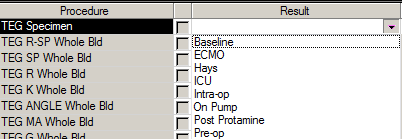
\includegraphics[width=.8\textwidth, trim={0, 27px, 0, 0}, clip]{graphics/specimen_type}
\end{minipage}

\clearpage
\paragraph{Enter the \textbf{measured}} results. in the spots provided.\marginnote{Note that the R-SP values should be skipped over. These results are calculated when both the R and SP have been entered. }\\
\vspace{.5em}
\begin{minipage}{\textwidth}
 \begin{tikzpicture}
\begin{scope}%[xshift=1.5cm]
    \node[anchor=south west,inner sep=0] (image) at (0,0) {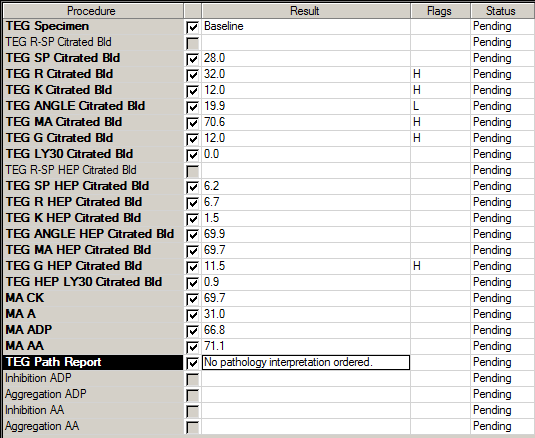
\includegraphics[width=\textwidth, trim={0, 27px, 0, 0}, clip]{graphics/results_entered}};
    \begin{scope}[x={(image.south east)},y={(image.north west)}]
        \draw [-stealth, line width=3pt, teal400] (1,1) to[out=178, in=0] (0.5,0.58);
        \draw [-stealth, line width=3pt, teal400] (1,1) to[out=178, in=0] (0.5,0.9);
    \end{scope}
\end{scope}
\end{tikzpicture}%
\end{minipage}\marginnote{Hitting `Enter' after typing a result will move you to the next field. }


\paragraph{Double Click } on the TEG Path Report's result field to open the Text Result window.\\
\vspace{.5em}
\begin{minipage}{\textwidth}
 % trim={<left> <lower> <right> <upper>}
 \IfFileExists{fileA.tex}{\input{fileA.tex}}
  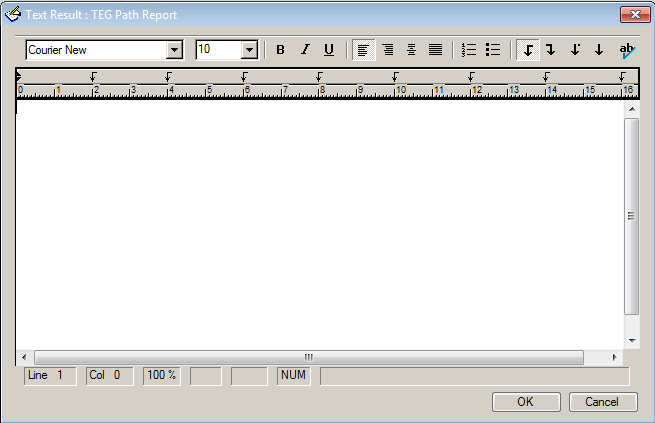
\includegraphics[width=.8\textwidth, trim={0, 0px, 0, 0}, clip]{graphics/text_result}
\end{minipage}

\newthought{If Pathology interpretation} \textbf{is} requested\\
\begin{description}
      \item Type ``path'' and hit the \textbf{F9} key to expand the Pathology template.
      \item Hit \textbf{F3} to move to case number field.
      \item Type the case number.
      \item Click 
\includegraphics[height=1em]{graphics/ok_button.png}  when finished.
\end{description}
\clearpage
\newthought{If Pathology interpretation} is \textbf{not} requested\\
\begin{description}
      \item Type ``npio'' and hit the \textbf{F9} key to expand the No Pathology template..
      \item Click 
\includegraphics[height=1em]{graphics/ok_button.png}  when finished.
\end{description}

\paragraph{Review} the results to ensure they've been entered correctly.\marginnote{Results can be held by clicking 
\includegraphics[height=1em]{graphics/perform.png}}
\paragraph{Verify} the results by clicking 
\includegraphics[height=1em]{graphics/verify.png}\marginnote{The Platelet mapping calculations will not trigger until the 
\includegraphics[height=1em]{graphics/verify.png} button is pressed.
}

\bigskip
\section{MA-A Corrections}
\newthought{if the MA-A} is >20.0 Cerner will send a Discern Notification shortly after the results have been verified.\\
\vspace{.5em}
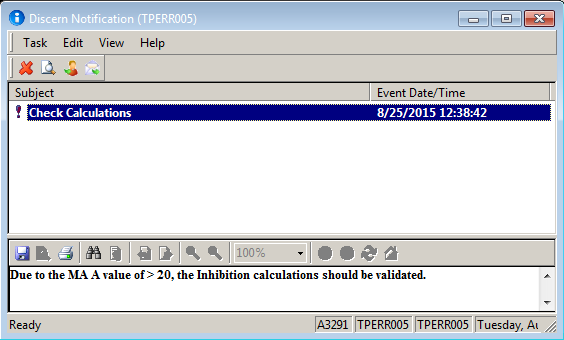
\includegraphics[width=.8\linewidth]{graphics/discern_notification.png}\marginnote[-4\baselineskip]{ The corrected results, along with the Accession Number will be displayed on the bottom pane of the Discern Notification.}

\newthought{At this point,} opening Accession Result Viewer again will show the platelet mapping results.\\
\vspace{.5em}
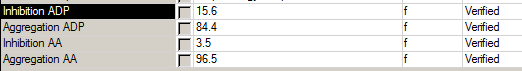
\includegraphics[width=\linewidth]{graphics/platelet_mapping_results}

\newthought{After reviewing } the corrected values, you can dismiss the notification.
\vspace{1em}
\marginnote[4\baselineskip]{Cerner will not allow you to close the window using the 
\includegraphics[height=1em]{graphics/discern_window_close}}
\begin{description}
    \item Click the 
\includegraphics[height=1em, trim={0, 0px, 0, 4px}, clip]{graphics/discern_close} icon to dismiss the notification\\
    \vspace{.5em}
    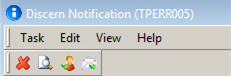
\includegraphics[width=.5\linewidth, trim={0, 0px, 0, 0px}, clip]{graphics/discern_toolbar}
    \item Click the 
\includegraphics[height=1em, trim={0, 0px, 0, 0px}, clip]{graphics/discern_minimize} hide the Discern Notification Window\\
    \vspace{.5em}
    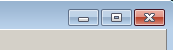
\includegraphics[width=.5\linewidth, trim={0, 0px, 0, 0px}, clip]{graphics/discern_window_buttons}
\end{description}

